\chapter{Background}
\label{chap:background}

\epigraph{A honeypot is a security resource whose value lies in being probed, attacked, or compromised.}{\textit{Lance Spitzner}}

Using honeypots in a cloud environment merges two varying principles.
This chapter introduces the fundamental knowledge needed to comprehend the upcoming experiments.
If the reader has a profound understanding of cloud computing, honeypots, and virtualization, he can skip this chapter.

% ====================================================================================================================
% Virtualization
\section{Virtualization}

Virtualization, often referred to as \acp{vm}, is defined by \citet{kreuter2004} as \enquote{an abstraction layer or environment between hardware component and the end-user}.
A \ac{vm} runs on top of the \acg{os} core components.
Through an abstraction layer, the \acl{vm} is connected with the real machine by hypervisors or \ac{vmm}.
Hypervisors can use real machine hardware components but also support \aclg{vm} operating systems and configurations.
Both are similar to emulators, which are defined by \citet{lichstei1969} as a \enquote{process whereby one computer is set up to permit the execution of programs written for another computer}.
This allows managing multiple \acp{vm} with real machine resources.
There are three different types of virtualization,
\begin{enumerate*}[label=(\roman*)]
    \item software virtual machines,
    \item hardware virtual machines, and
    \item virtual OS/containers
\end{enumerate*}.
Software virtual machines manage interactions between the host and guest operating systems.
Hardware virtual machines offer direct and fast access to the underlying resources.
It uses hypervisors, modified code, or APIs.
Lastly, virtual OS/container partitions the host operating system into containers or zones.
\cite{daniels2009}

% ====================================================================================================================
% Cloud Computing
\section{Cloud Computing}
\label{sec:cloud-computing}

Cloud Computing has become a viral keyword these days.
It has been used by various large companies such as Google and Amazon.
However, the term \enquote{cloud computing} dates back to late 1996, when a small group of technology executives of Compaq Computer framed new business ideas around the Internet.\cite{regalado2020}
Starting from 2007, cloud computing evolved into a serious competitor and outnumbered the keywords' \enquote{virtualization}, and \enquote{grid computing} as reported by Google trends \cite{Wang2010}.
Shortly, various cloud providers become publicly available, each with its strengths and weaknesses.
For example IBM's Cloud\footnote{\url{https://www.ibm.com/cloud}}, Amazon Web Services\footnote{\url{https://aws.amazon.com/}}, and Google Cloud\footnote{\url{https://cloud.google.com/}}.
Why are clouds so attractive in practice?

\begin{itemize}
    \item It offers major advantages in terms of cost and reliability.
    When demand is needed, consumers do not have to invest in hardware when launching new services.
    Pay-as-you-go allows flexibility.
    \item Consumers can easily scale with demand.
    When more computational resources are required due to more requests, scaling up instances in conjunction with a suited price model is straightforward.
    \item Geographically distributed capabilities supply the need for worldwide scattered services.
\end{itemize}

% ====================================================================================================================
% Definition of cloud computing
\subsection{Definition of Cloud Computing}

Concerning the definition by Brian Hayes, cloud computing is \enquote{a shift in the geography of computation} \cite{hayes2008}.
Thus, the computational workload is moved away from local instances towards services and data centers that provide the user's needs\cite{Armbrust2010}.

The \ac{nist} defines cloud computing as \enquote{a model for enabling ubiquitous, convenient, on-demand network access to a shared pool of configurable computing resources (e.g., networks, servers, storage, applications, and services) that can be rapidly provisioned and released with minimal management effort or service provider interaction} \cite{Mell2011}.
\ac{nist} not only reflects the geographical shift of resources such as data centers but also mentions on-demand usage that contributes to flexible resource management.
Moreover, \ac{nist} composes the term in five essential characteristics, three service models (see \autoref{subsec:cloud-service}), and four deployment models (see \autoref{subsec:cloud-deployment}) \cite{Mell2011}

\textit{On-demand-self-service} refers to the unilateral provision computing capabilities.
Consumers can acquire server time and network storage on demand without human interaction.

\textit{Broad network access} characterizes the access of capabilities of the network through standard protocols such as \acs{http}.
Heterogeneous thin and thick client platforms should be supported.

\textit{Resource pooling} allows the provider's computing resources to be pooled across several consumers.
Different physical and virtual resources are assigned on-demand with a multi-tenant model.
Other aspects such as location are independent and cannot be controlled on a low level by consumers.
Moreover, high-level access to specify continent, state, or datacenter can be available.

\textit{Rapid elasticity} offers consumers to extend and release capabilities quickly.
Further automation to quickly increase resources when demand surges can be supported at any time, regardless of limit or quantity.

\textit{Measured service} handles resources in an automated and optimized manner.
It uses additional metering capabilities to trace storage, processing, bandwidth, and active user accounts.
This helps to monitor and control resource usage.
Thus, contributing to transparency between provider and consumer.

% ====================================================================================================================
% Service models
\subsection{Service models}
\label{subsec:cloud-service}

Service models are categorized by \ac{nist} into three basic models based on usage and abstraction level.
\autoref{fig:cloud-functionalities} shows the connection between each model whereas cloud resource are defined in \autoref{subsec:cloud-deployment}.
\ac*{iaas} builds with a vast range of functionalities the foundation of service models.
Each model on top represents a user-friendly abstraction with derated capabilities.

\begin{figure}
    \centering
    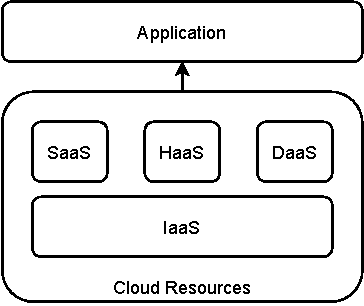
\includegraphics[width=0.4\textwidth]{figures/cloud-service-models.pdf}
    \caption[Abstract visualization of service models]{
        Abstract visualization of service models.
        The lowest level within the container \enquote{cloud resources} represents the depth of functionalities.
        Therefore, \ac{iaas} offers the most functionalities, whereas the others have a user-friendly abstraction.
    }
    \label{fig:cloud-functionalities}
\end{figure}

\ac{saas} is a high-level abstraction to consumers.
Controlling the underlying infrastructure is not supported.
Providers often use a multi-tenancy system architecture to organize each consumer's application in a different environment.
It helps to employ scaling with respect to speed, security availability, disaster recovery, and maintenance.
The main objective of \ac{saas} is to host a consumer's software or application that can be accessed over the Internet using either a thin or rich client. \cite{Dillon2010}
\enquote{Limited user-specific application configuration settings} can be made \cite{Mell2011}.

\ac{paas} pivots on the full \enquote{Software Lifecycle} of an application whereas \ac{saas} distinct on hosting complete applications.
\ac{paas} offers ongoing development and includes programming environment, tools, configuration management, and other services.
In addition, the underlying infrastructure is not managed by the consumer. \cite{Mell2011}

\ac{iaas} offers a low-level abstraction to consumers with the ability to run arbitrary software regardless of the operating system or application.
In contrast to \ac{saas}, IT infrastructure capabilities (such as storage, networks) can be used.
It strongly depends on virtualization due to the integration or decomposition of physical resources. \cite{Mell2011}

\ac{daas} serves as a virtualized data storage service on demand.
Motivations behind such services could be upfront costs of on-premise enterprise database systems. \cite{Dillon2010}
Mostly they require \enquote{dedicated server, software license, post-delivery services, and in-house IT maintenance} \cite{Dillon2010} whereas \ac{daas} costs solely what consumers need.
When dealing with a tremendous amount of data, file systems and RDBMS often lack performance.
\ac{daas} outruns such weak links by employing a table-style abstraction that can be scaled. \cite{Dillon2010}

\ac{haas} offers IT hardware or datacenters to buy as a pay-as-you-go subscription service.
The term dates back to 2006 when hardware virtualization became more powerful.
It is flexible, scalable, and manageable. \cite{Wang2010}

% ====================================================================================================================
% Deployment models
\subsection{Deployment models}
\label{subsec:cloud-deployment}

Deployment models are categorized by \ac{nist} into four basic models.
Each differs in data privacy, location, and manageability \cite{Mell2011}.

With private clouds, users have the highest control regarding data privacy and utilization.
Such clouds are mostly deployed within a single organization, managed by in-house teams or third-party suppliers.
In addition, it can be on- or off-premise.
Within private clouds, consumers have full control of their data.
Especially for European data privacy laws, it is not negligible when data is stored abroad, and thus, under the law of foreign countries.
However, its popularity has not been diminished due to the immense cost of switching to public clouds. \cite{Dillon2010, Mell2011}

Community clouds can be seen as a conglomerate of multiple organizations that merge their infrastructure with respect to a commonly defined policy, terms, and conditions beforehand. \cite{Mell2011}

Public clouds represent the most used deployment models.
Contrary to private ones, public clouds are fully owned by service providers such as businesses, academics, or government organizations.
Consumers do not know where their data is distributed.
In addition, contracts underlie custom policies. \cite{Mell2011}

A hybrid cloud mixes two or more cloud infrastructures, such as private and public clouds.
However, each entity keeps its core element.
Hybrid clouds define \enquote{standardized or proprietary technology to enable data and application portability}\cite{Mell2011}.

% ====================================================================================================================
% Honeypots
\section{Honeypots}

The term \enquote{honeypot} has been established for more than two decades.
1997 was the first time that a free honeypot solution became public.
\ac{dtk}, developed by Fred Cohen, released the first honeypot solution.
However, the earliest drafts of honeypots are from 1990/91 and built the foundation for Fred Cohen's \ac*{dtk}.
Clifford Stoll's book \enquote{The Cuckoo's Egg}\cite{stroll2000}, and Bill Cheswick's whitepaper \enquote{An Evening With Berferd}\cite{Cheswick92} describe concepts that are considered nowadays as honeypots.\cite{Spitzner2003}
A honeypot itself is a security instrument that collects information on buzzing attacks.
It disguises itself as a system or application with weak links, so it gets exploited and gathers knowledge about the adversary.
In 2002, a Solaris honeypot helped to detect an unknown \verb|dtspcd| exploit.
Interestingly, a year before in 2001 the Coordination Center of \acs{cert}\footnote{\acl{cert} is an expert group that handles computer security incidents\cite{cert2021}} shared their concerns regarding the dtspcd.
Communities were aware that the service could be exploited to get access and remotely compromise any Unix system.
However, such an exploit was not known during this time, and experts did not expect any in the near future.
Luckily, early instances based on honeypot technologies could detect new exploits and avoid further incidents.
Such events emphasize the importance of honeypots.

% ====================================================================================================================
% Definition of a honeypot
\subsection{Definition of Honeypots}

Many definitions for honeypots circulate through the web that causing confusion and misunderstandings.
In general, the objective of a honeypot is to gather information about attacks or attack patterns \cite{NawrockiWSKS2016}.
Thus, contributing as an additional source of security measure.
See \autoref{subsec:honeypot-security-concept} for a detailed view regarding honeypots in the security concept.
As \citet{Spitzner2003} has listed, the most misleading definitions are: a honeypot is a tool for deception, it is a weapon to lure adversaries or a part of an intrusion detection system.
In order to get a basic understanding, this section wants to exhibit some key definitions.
\citet{Spitzner2003} defines honeypots as a \enquote{security resource whose value lies in being probed, attacked, or compromised}.
Independent of its source (e.g., server, application, or router), he expects the instance to be probed, attacked, and eventually exploited.
If a honeypot does not match this behavior, it will not provide any value.
It is essential to mention that honeypots do not have any production value; thus, any communication that is acquired is suspicious by nature \cite{Spitzner2003}.
In addition, \citet{Spitzner2003} points out that honeypots are not bound to solve a single problem; hence, they function as a generic perimeter and fit into different situations.
Such functions are attack detection, capturing automated attacks, or alert/warning generators.
\autoref{fig:honeypot-example} shows an example of how honeypots could be used in an IT infrastructure.

\begin{figure}
    \centering
    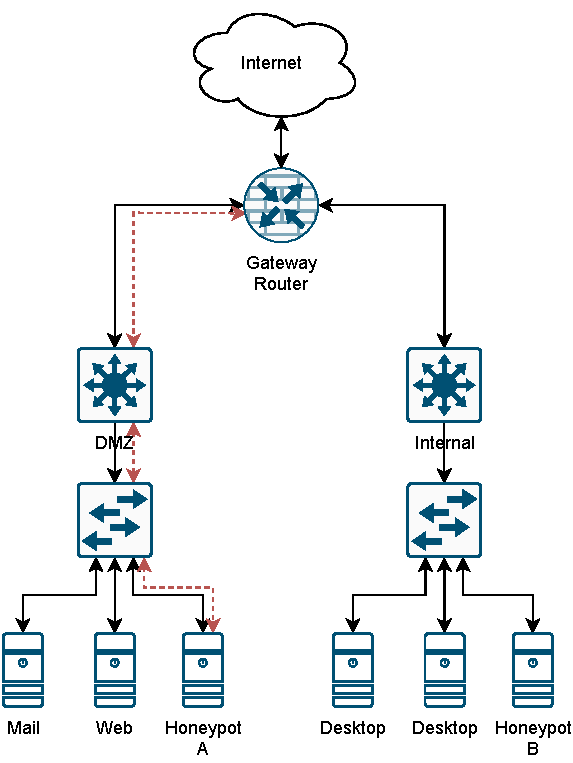
\includegraphics{figures/honeypot-example.pdf}
    \caption[Example of honeypots in a simplified network]{
        Example of honeypots in a simplified network (derived from \cite{Spitzner2003}).
        Each of the \acp{dmz} and internal networks are separated by a router and a Layer-3 switch.
        As derived from above, in each network a honeypot is available (honeypot A, B).
        The red path symbolizes the path of an attacker coming from the gateway router.
    }
    \label{fig:honeypot-example}
\end{figure}

In general, it differentiates two types of honeypots
\begin{enumerate*}[label=(\roman*)]
    \item production honeypots
    \item research honeypots
\end{enumerate*}.
This categorization has its origin from Mark Rosch, a developer of Snort, during his work at GTE Internetworking. \cite{vetterl2020}

Production honeypots are the common type of honeypots that people would think of.
The objective is to protect production environments and mitigate the risk of attacks.
Usually, production honeypots are easy to deploy within an organization.
Mostly, low-interaction honeypots are chosen due to a significant risk reduction, so adversaries cannot exploit honeypots to attack other systems.
The downside of a low-interaction honeypot is a lack of information, which means only standard information like the origin of attacks or what exploits have been used can be collected.
In contrast, insides about communication of attackers or deployment of such attacks are unlikely to obtain.
In contrast, research honeypots do fulfill this objective. \cite{Spitzner2003}

Research honeypots are used to learn more in detail about attacks.
The objective is to collect information about clandestine organizations, new tools for attacks, or the origin of attacks.
Research honeypots are unlikely suitable for production environments due to a higher risk increase.
Facing an increase in deployment complexity and maintenance does not attract production usage either. \cite{Spitzner2003}

It is worth mentioning that there is no exact line between research or production honeypots.
A possible use case is a honeypot that functions as a production or a research honeypot.
Due to the dynamic range in which they are applicable, it is difficult to distinguish them.

In addition, \citet{Provos2003} adds a differentiation for the virtual honeypot framework and splits it into the following types:

\begin{itemize}
    \item Physical honeypots are \enquote{real machines on the network with its own IP address} \cite{Provos2003}
    \item Virtual honeypots are \enquote{simulated by another machine that responds to network traffic sent to the virtual honeypot} \cite{Provos2003}
\end{itemize}

% ====================================================================================================================
% Level of interaction
\subsection{Level of Interaction}
\label{subsec:interaction-honeypots}

When building and deploying a honeypot, the depth of information has to be defined beforehand.
Should it gather unauthorized activities, such as an \textsc{nmap} scan?
Do you want to learn about buzzing tools and tactics?
Each depth brings a different level of interaction because some information depends on more actions of adversaries.
Therefore, honeypots differ in their level of interaction.

Low-interaction honeypots provide the lowest level of interaction between an attacker and a system.
Only a small set of services like SSH, Telnet, or FTP are supported, contributing to the deployment time.
In terms of risk, a low-interaction honeypot does not give access to the underlying \ac{os} which makes it safe to use in a production environment.
For example, using an SSH honeypot with emulated services allows attackers to log in and execute commands by brute force or guesswork.
The adversary will never gain more access because it is not a real \ac{os}.
However, safety comes with the downside of less information.
The collection is limited for the statistical purpose such as
\begin{enumerate*}[label=(\roman*)]
    \item time and data of attack
    \item source IP address and source port of the attack
    \item destination IP address and destination port of the attack
\end{enumerate*}.
The transactional information can not be collected. \cite{Spitzner2003}

A medium-interaction honeypot offers more sophisticated services with a higher level of interaction.
It is capable of responding to specific activities.
For example, a Microsoft IIS Web server honeypot could respond in a way that a worm is expecting.
The worm would get emulated answers and could be able to interact with it in more detail.
In this way, more severe information about the attack can be gathered, including privilege assessment, toolkit capture, and command execution.
In comparison, medium-interaction honeypots allocate more time to install and configure.
Also, more security checks have to be performed due to a higher interaction level than low-interaction honeypots. \cite{Spitzner2003}

High-interaction honeypots represent a real \ac{os} to provide a full set of interactions to attackers.
They are so powerful because other production servers do not differ much from high-interaction honeypots.
They represent real systems in a controlled environment.
The amount of information is tremendous.
It helps to learn about
\begin{enumerate*}[label=(\roman*)]
    \item new tools
    \item finding new bugs in the \ac{os}
    \item the black hat community
\end{enumerate*}.
However, the risk of such a honeypot is extremely high.
It needs severe deployment and maintenance processes; thus, it is time-consuming.

% ====================================================================================================================
% security concepts
\subsection{Security concepts}
\label{subsec:honeypot-security-concept}

Security concepts are classified by \citet{Schneier2004} in prevention, detection, and reaction.
Prevention includes any process that
\begin{enumerate*}[label=(\roman*)]
    \item discourages intruders and
    \item hardens systems to avoid any breaches
\end{enumerate*}.
Detection scrutinizes the identification of attacks that threatens the systems'
\begin{enumerate*}[label=(\roman*)]
    \item confidentiality
    \item integrity and
    \item availability
\end{enumerate*}.
Reaction treats the active part of the security concept.
When attacks are detected, it conducts reactive measures to remove the threat.
Each part is designed to be sophisticated so that all of them contribute to a secure environment. \cite{NawrockiWSKS2016}

Honeypots contribute to the security concept like firewalls, or \acp{ids}.
However, honeypots add only a small value regarding prevention because security breaches cannot be identified.
Moreover, attackers would avoid wasting time on honeypots and go straight for production systems instead.

Detection is one of the strengths of honeypots.
Attacks often vanish in the sheer quantity of production activities.
If any connection is established to a honeypot, it is suspicious by nature.
In conjunction with an alerting tool, attacks can be detected.

Honeypots strongly supply reaction tools due to their clear data.
It is difficult to find attacks for further data analysis in production environments.
Often data submerge with other activities, which complicates the process of reaction. \cite{NawrockiWSKS2016}
\citet{NawrockiWSKS2016} distinguish honeypots from other objectives such as firewall or log-monitoring.

\begin{table}
    \centering
    \caption[Distinction between security concepts]{
        Distinction between security concepts based on areas of operations (derived from \cite{NawrockiWSKS2016}).
    }
    \begin{tabular}{l|lll}
        \toprule
        \textbf{Objective}        & \textbf{Prevention} & \textbf{Detection} & \textbf{Reaction} \\ \hline
        Honeypot                  & +                   & ++                 & +++               \\
        Firewall                  & +++                 & ++                 & +                 \\
        Intrusion Detection Sys.  & +                   & +++                & +                 \\
        Intrusion Prevention Sys. & ++                  & +++                & ++                \\
        Anti-Virus                & ++                  & ++                 & ++                \\
        Log-Monitoring            & +                   & ++                 & +                 \\
        Cybersecurity Standard    & +++                 & +                  & +                 \\
        \bottomrule
    \end{tabular}
    \label{tab:honeypots-security-concepts}
\end{table}

% ====================================================================================================================
% Value of honeypots
\subsection{Value of Honeypots}

To assess the value of honeypots, this section looks at their advantages and disadvantages. \cite{Mokube2007,Kaur2014,Spitzner2003}

\subsubsection{Advantages}

\begin{itemize}
    \item \textit{Data Value}: Collected data is often immaculate and does not contain noise from other activities.
          Thus, reducing the total data size and speeding up the analysis.
    \item \textit{Resources}: Firewalls and \ac{ids} are often overwhelmed by the gigabits of traffic, thus, dropping network packets for analysis.
          This results in far less effective detection of malicious network activities.
          However, honeypots are independent of resources because they only capture their activities.
          Due to resource limitations, expensive hardware is not needed.
    \item \textit{Simplicity}: A honeypot does not require complex algorithms or databases.
          A user should be able to deploy it somewhere quickly.
          Research honeypots might come with an inevitable increase of complexity.
          However, if a honeypot is complex, it will lead to misconfigurations, breakdowns, and failures.
    \item \textit{Return on Investment}: Capturing attacks immediately informs users that suspicious activities occur on the infrastructure.
          This helps to demonstrate their value and contributes to new investments in other security measurements.
\end{itemize}

In addition, \citet{NawrockiWSKS2016} listed four more advantages of honeypots:

\begin{itemize}
    \item \textit{Independent of Workload}: Honeypots only process traffic directed to them.
    \item \textit{Zero-Day-Exploit Detection}: It helps to detect unknown strategies and zero-day-exploits.
    \item \textit{Flexibility}: Well-adjusted honeypots for various specific tasks are available.
    \item \textit{Reduced False Positives and Negatives}: Any traffic or connection to a honeypot is suspicious.
          Client-honeypots verify such attacks based on system state changes.
          This results in either false positive or false negatives.
\end{itemize}

\subsubsection{Disadvantages}

\begin{itemize}
    \item \textit{Narrow Field of View}: Only direct attacks on honeypots can be investigated, whereas attacks on the production system are not detected.
    \item \textit{Fingerprinting}: A honeypot often has a certain fingerprint that attackers can identify.
          Especially commercial ones can be detected by their responses or behaviors.
    \item \textit{Risk to the Environment}: Using honeypots in an environment always increases risk.
          However, it depends on the level of interaction.
\end{itemize}

\subsection{Honeynets}

Instead of having single honeypots that can be attacked, a honeynet offers a complete network of standard production systems such as you would find in an organization.
Those systems are high-interaction honeypots, thus, allowing them to fully interact with the \ac{os} and applications.
The key idea is that an adversary can probe, attack, and exploit these systems so that the maintainer can derive interaction within this network.
It should be mentioned that a honeynet has to be protected by firewalls.
For example, \autoref{fig:honeynet-example} represents such a honeynet within an organization.

\begin{figure}
    \centering
    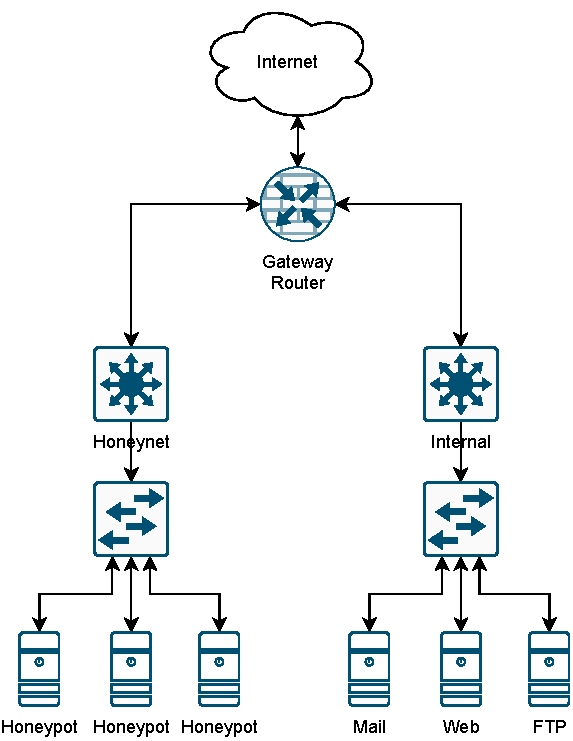
\includegraphics{figures/honeynet-example.pdf}
    \caption[Example of honeynets in a simplified network]{
        Example of honeynets in a simplified network (derived from \cite{Spitzner2003}).
        This network presents the honeynet consisting of several other honeypots on the left.
        On the right, the network presents a common subnet consisting of mail, web, and FTP server.
    }
    \label{fig:honeynet-example}
\end{figure}

Compared to a traditional honeypot, the most significant value of honeynets is the usage of proper production systems.
Black hats often do not know that they attack a honeynet, thus, adding value to prevention.
However, the downsides are the high complexity and maintenance needed to keep a honeynet running. \cite{Spitzner2003}

% ====================================================================================================================
% Legal issues
\subsection{Legal Issues}

Considering questions related to legal issues of honeypots can easily exceed this thesis.
In this regard, this section restricts the study to the country the author resides in.
Thus, it is only concerned about the \ac{eu} regulations, EU directives, and international agreements.
Honeypots collect
\begin{enumerate*}[label=(\roman*)]
    \item content data that is used for communication, and
    \item transactional data that is used to establish the connection
\end{enumerate*}.
\citet{sokol2017} studied the legal conditions for data collection and data retention.
They have concluded that administrators of honeypots have a legal ground of legitimate interest to store and process personal data, such as IP addresses.
Moreover, for production honeypots, the legitimate interest is to secure services.
Regarding the length of data retention, the principle of data minimization has to be considered, which means there is no clear answer.
Any published data of research honeypots needs to be anonymized.
